\newpage
\section{Metodologia Experimental}

\subsection{Materiais}

Para a realização do experimento foi utilizado o software Simulink do pacote 
Matlab.

\subsection{Métodos}
O experimento foi realizado em simulações. De início, foi estudado o 
comportamento da modulação PAM com sinalização duobinário. Em seguida, foi analisada a modulação PAM com sistema duobinário modificado.

O próximo passo foi obter o desempenho de ambos os métodos em um canal AWGN simples.

Por ultimo, foi obtido a densidade espectral de potência para as duas técnicas de sinalização.

As seções seguintes dão mais detalhes sobre o procedimento.

\subsubsection{Simulação do PAM Duobinário}
Na primeira atividade, foi montado o circuito da figura \ref{fig:simdb}. Os parâmetros de cada bloco são apresentados logo abaixo.

\begin{figure}[H]
    \centering
    \caption{Diagrama do sistema com modulação PAM duobinário.}
    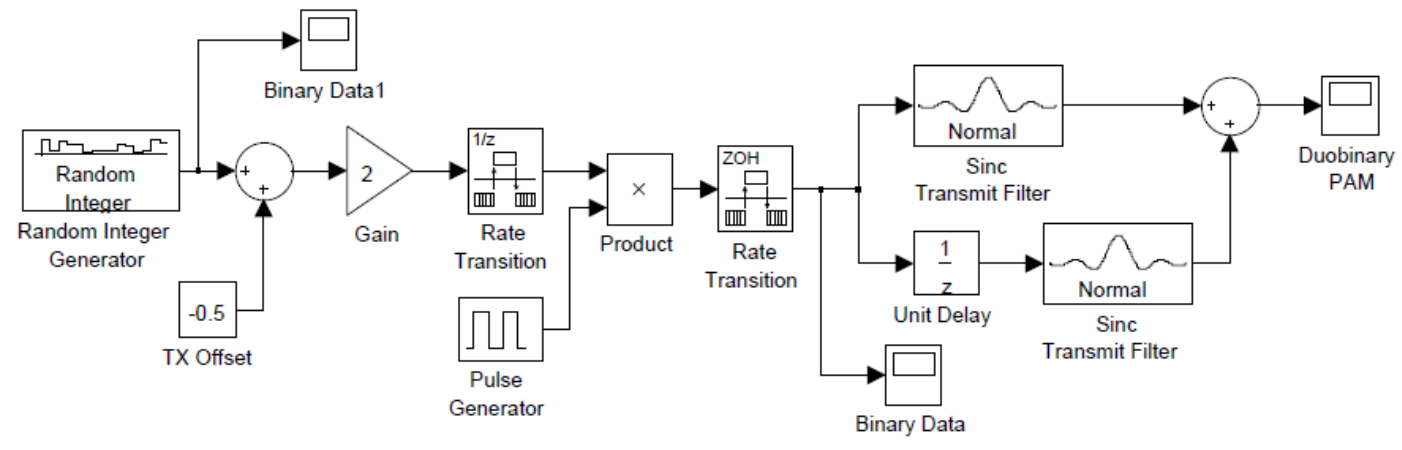
\includegraphics[scale=0.3]{simdb}
    \label{fig:simdb}
\end{figure}
  
\textbf{A – Random Integer Generator} – Communications blockset; Comm Sources

PARÂMETROS: - M-ary number: 2; Initial seed: randseed; Sample time: 1e-3; Output data type: double.

\textbf{B – Sum} – Simulink blockset; Math Operations

PARÂMETROS: - Main: Icon shape: rectangular; List of signs: I++; Sample time (-1 for inherited): -1.

\textbf{C – Constant} – Simulink blockset; Source

PARÂMETROS: - Main: Constant value: -0.5; [x] Interpret vector parameters as 1-D; Sample time: inf.

\textbf{D – Gain} – Simulink blockset; Math Operations

PARÂMETROS: - Main: Gain: 2; Multiplication: Element-wise(k.*u); Sample time (-1 for inherited): -1.

\textbf{E – Rate Transition} – Simulink Blockset; Signal Attributes

PARÂMETROS: [x] Ensure data .....; [x] Ensure deterministic...; Initial Conditions: 0; Output port sample time options: Specify; Output port Sample time: 2e-5.

\textbf{F – Pulse Generator} – Simulink Blockset; Sources

PARÂMETROS: Pulse type: Time based; Time (t): Use simulation time; Amplitude: 1; Period (secs): 1e-3; Pulse Width(\% of period): 2; Phase Delay(s): 0; [x] Interpret vector parameters as 1-D. 

\textbf{G – Product Block} – Simulink Blockset; Math Operations.

PARÂMETROS: Main: Number of imputs:2; Multiplication: Element-wise; Sample time: -1.

\textbf{H – Rate Transition} – Simulink Blockset; Signal Attributes

PARÂMETROS: [x] Ensure data .....; [x] Ensure deterministic...; Initial Conditions: 0; Output port sample time options: Specify; Output port Sample time: 1e-3.

\textbf{I – Raised Cosine Transmiter Filter} – Communication Blockset; Comm Filters

PARÂMETROS: Main: Filter type: Normal; Group delay (number of symbols): 4; Rollof factor (0 to 1): 0; Upsampling factor (N): 50; Input processing: Inherited (this choi.....); Rate options: Allow multirate processing; Filter gain: User-specified; Linear amplitude filter gain: 5.

\textbf{J – Unit Delay} – Simulink blockset; Math Operations

PARÂMETROS: - Main: Initial conditions: 0; Input processing: Inherited; Sample time (-1 for inherited): -1.

\textbf{K – Raised Cosine Transmiter Filter} – Communication Blockset; Comm Filters

PARÂMETROS: Main: Filter type: Normal; Group delay (number of symbols): 4; Rollof factor (0 to 1): 0; Upsampling factor (N): 50; Input processing: Inherited (this choi.....); Rate options: Allow multirate processing; Filter gain: User-specified; Linear amplitude filter gain: 5 (ou (5)*rcfiltgaincompat(gcbh) novas versões).

\textbf{L – Sum} – Simulink blockset; Math Operations

PARÂMETROS: - Main: Icon shape: round; List of signs: I++; Sample time (-1 for inherited): - 1.

Os parâmetros de simulação são:

\begin{lstlisting}[language=matlab]
  Configuration Parameters: 
  Start time: 0; 
  Stop time: 0.05; 
  Type: Fixed-step; 
  Solver: ode3;  
  Fixed-step size: 2e-5; 
  Periodic sample time constraint: Unconstrained; 
  Tasking mode for periodic sample times: Auto.
\end{lstlisting}

Foram obtidos os gráficos nos pontos com osciloscópio e foi analisado o funcionamento do sistema.

\subsubsection{Simulação do PAM Duobinário Modificado}

Na segunda atividade, foi montado o circuito da figura \ref{fig:simmdb}. Os parâmetros de cada bloco são apresentados logo abaixo.

\begin{figure}[H]
  \centering
  \caption{Diagrama do sistema com modulação PAM duobinário modificado.}
  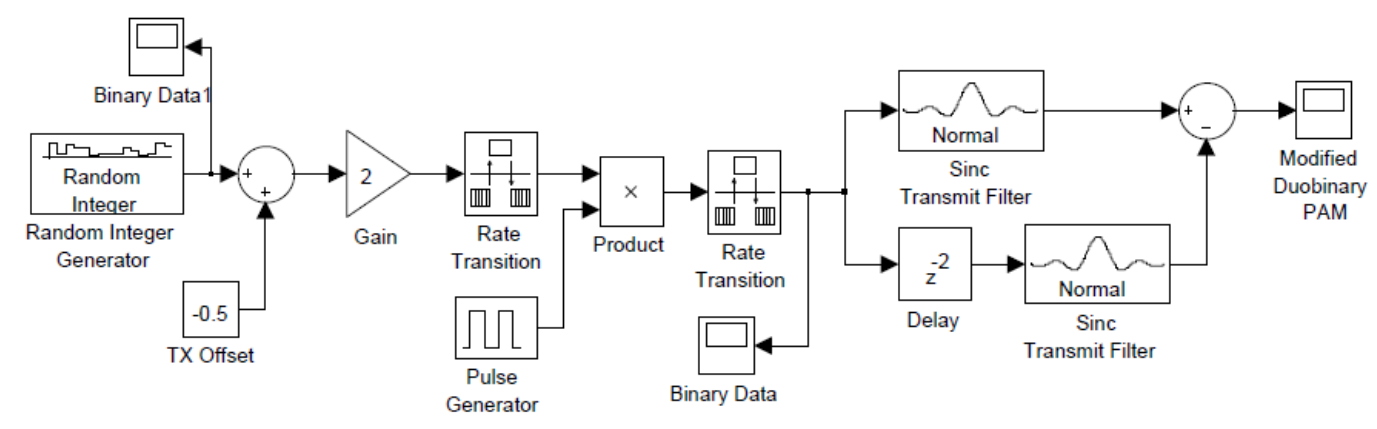
\includegraphics[scale=0.3]{simmdb}
  \label{fig:simmdb}
\end{figure}

\textbf{A – Delay} – Signal Processing blockset; Signal Operations

PARÂMETROS: - Input processing: Inherited; Delay units: Samples; Delay (samples): 2; Initial conditions: 0; Reset port: None.

\textbf{B – Sum} – Simulink blockset; Math Operations 

PARÂMETROS: - Main: Icon shape: round; List of signs: I+-; Sample time (-1 for inherited): - 1.

Foram obtidos os gráficos nos pontos com osciloscópio e foi analisado o funcionamento do sistema.


\subsubsection{Desempenho para o PAM Duobinário em um Receptor Simples no Canal AWGN}

Em seguida foi analisado o desempenho do PAM duobinário em um receptor simples no canal AWGN. Para isso foi montado o sistema da figura \ref{fig:simdbawgn}

\begin{figure}[H]
  \centering
  \caption{Diagrama do sistema com modulação PAM duobinário e receptor simples.}
  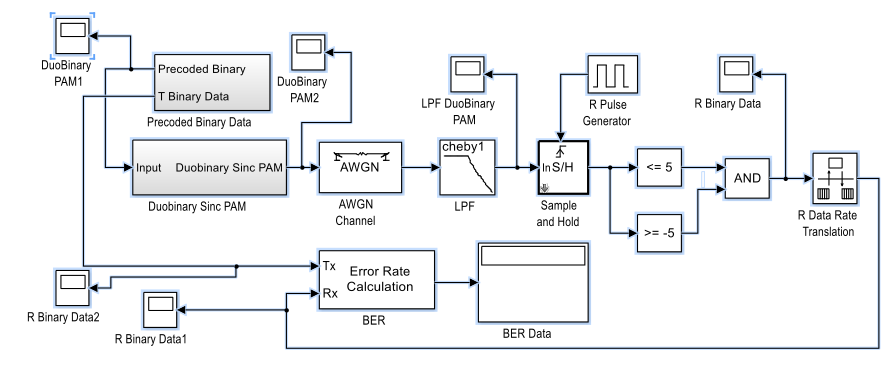
\includegraphics[scale=0.5]{simdbawgn}
  \label{fig:simdbawgn}
\end{figure}

Os parâmetros dos blocos são:

\textbf{A – AWGN} – Communications Blockset; Channels 

PARÂMETROS: Input processing: Inherited; Initial seed: randseed; Mode: Variance from mask; Variance: 200.

\textbf{B - Analog Filter Design} – Signal Processing Blockset; Filters Designs

PARÂMETROS: Design method: Chebyshev I; Filter type: Lowpass; Filter order: 9;
Passband edge frequency (rad/s): 2*pi*600; Passband ripple in dB: 0.1.

\textbf{C – Sample and Hold} – Signal Processing Blockset; Signal Operations

PARÂMETROS: Trigger type: Rising edge; Initial condition: 0.

\textbf{D – Pulse Generator} – Simulink Blockset; Sources

PARÂMETROS: Pulse type: Time based; Time (t): Use simulation time; Amplitude: 1; Period (secs): 1e-3; Pulse Width(\% of period): 2; Phase Delay(s): 0; [x] Interpret vector parameters as 1-D.

\textbf{E – Compare to Constant} –Simulink Blockset; Logic and Bitwise Operations

PARÂMETROS: Operator: <=; Constant value: 5; Output data type mode: Boolean.

\textbf{F – Compare to Constant} –Simulink Blockset; Logic and Bitwise Operations

PARÂMETROS: Operator: >=; Constant value: -5; Output data type mode: Boolean.

\textbf{G – Logical Operator} – Simulink blockset; Logic and Bitwise Operations

PARÂMETROS: Main: Operator: AND; Number of imput ports: 2; Icon shape: rectangular; Sample time (-1 for inherited): -1. Signal Attributes: Output data type: Boolean.

\textbf{H – Rate Transition} – Simulink Blockset; Signal Attributes

PARÂMETROS: [x] Ensure data .....; [x] Ensure deterministic...; Initial Conditions: 0; Output port sample time options: Specify; Output port Sample time: 1e-3.

\textbf{I – Error Rate Calculation} – Communications Blockset – Comm Sinks

PARÂMETROS: Receive Delay: 8; Computation delay: 1; Computation mode: Entire frame; Output data: Port.
\\
\begin{figure}[H]
  \centering
  \caption{Pré-codificação doubinário.}
  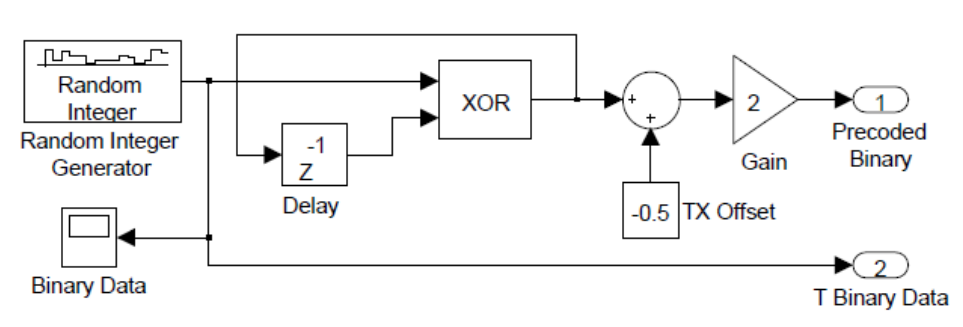
\includegraphics[width=\textwidth]{simdbprecode}
  \label{fig:simdbprecode}
\end{figure}

O sistema de pré-codificação da figura \ref{fig:simdbprecode} tem os parâmetros descritos abaixo.

\textbf{A – Random Integer Generator	} – Communications blockset; Comm Sources

PARÂMETROS: - M-ary number: 2; Initial seed: randseed; Sample time: 1e-3; Output data type: boolean.

\textbf{B – Integer Delay} – Signal Processing blockset; Signal Operations

PARÂMETROS: - Number of delays: 1; Input processing: Inherited; Initial conditions: 0.0; Sample time: -1.

\textbf{C – Logical Operator} – Simulink blockset; Logic and Bitwise Operations

PARÂMETROS: Main: Operator: XOR; Number of imput ports: 2; Icon shape: rectangular; Sample time (-1 for inherited): -1. Signal Attributes: Output data type: Boolean.

Os parâmetros de simulação são:

\begin{lstlisting}[language=matlab]
Configuration Parameters: 
Start time: 0; 
Stop time: 0.05; 
Type: Fixed-step; 
Solver: ode3;  
Fixed-step size: 2e-5; 
Periodic sample time constraint: Unconstrained; 
Tasking mode for periodic sample times: Auto.
\end{lstlisting}

Obeter:
\begin{enumerate}
  \item gráfico nos pontos onde possui o osciloscópio. Explicar o seu funcionamento através da comparação entre gráficos;
  
  \item verificar o atraso no sinal recebido em relação ao transmitido;
  
  \item preencher a tabela \ref{tab:simdb} com os dados da simulação;
  
  \item plotar o gráfico BERxSNR com um LPF (9 polos Chebyshev, 0,1 dB de ripple, freq. Corte de 600 Hz) em um sistema de comunicação digital PAM sinc duobinário precodificado com potência do sinal normalizada 50,6W.
\end{enumerate}

\begin{table}[H]
  \begin{center}
    \caption{Tabela BER x Eb/No para PAM duobinário.}
    \begin{tabular}{|c|c|c|}
      \hline
      SNR (dB) & AWGN $\sigma^2 (V^2)$ & BER \\
      \hline
      7,04 & 10 & 0 \\
      \hline
       & 50 & 0.0243 \\
      \hline
       & 100 & \\
      \hline
       & 200 & \\
      \hline
       & 300 & \\
      \hline
       & 400 & \\
      \hline 
       & 500 & \\
      \hline
    \end{tabular}
    \label{tab:simdb}
  \end{center}
\end{table}

\subsubsection{Desempenho para o PAM Duobinário Modificado em um Receptor Simples no Canal AWGN}

O transmissor PAM sinc duobinário modificado, o canal de comunicação e o receptor PAM simples são similares ao do sistema de comunicação PAM sinc duobinário precodificado. A figura \ref{fig:simmdbawgn} mostra o diagrama de blocos simulado.

\begin{figure}[H]
  \centering
  \caption{Diagrama do sistema com modulação PAM duobinário modificado e receptor simples.}
  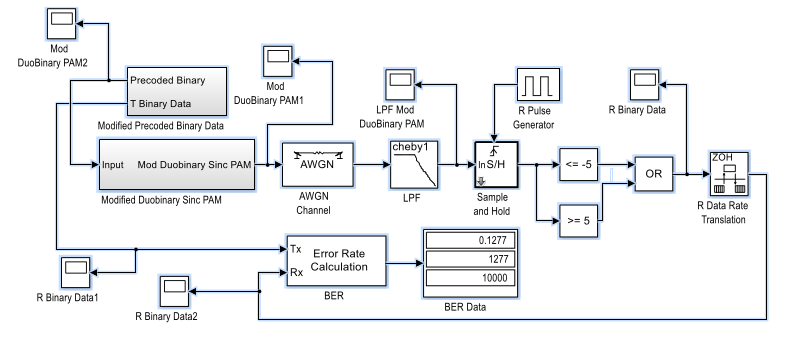
\includegraphics[scale=0.5]{simmdbawgn}
  \label{fig:simmdbawgn}
\end{figure}

Os parâmetros dos blocos são:

\textbf{A – Compare to Constant} –Simulink Blockset; Logic and Bitwise Operations

PARÂMETROS: Operator: <=; Constant value: -5; Output data type mode: Boolean.

\textbf{B – Compare to Constant} –Simulink Blockset; Logic and Bitwise Operations

PARÂMETROS: Operator: >=; Constant value: 5; Output data type mode: Boolean.

\textbf{C – Logical Operator} – Simulink blockset; Logic and Bitwise Operations

PARÂMETROS: Main: Operator: OR; Number of imput ports: 2; Icon shape: rectangular; Sample time (-1 for inherited): -1. Signal Attributes: Output data type: Boolean.

\textbf{D – Error Rate Calculation} – Communications Blockset – Comm Sinks

PARÂMETROS: Receive Delay: 8; Computation delay: 2; Computation mode: Entire frame; Output data: Port.

\begin{figure}[H]
  \centering
  \caption{Pré-codificação doubinário modificado.}
  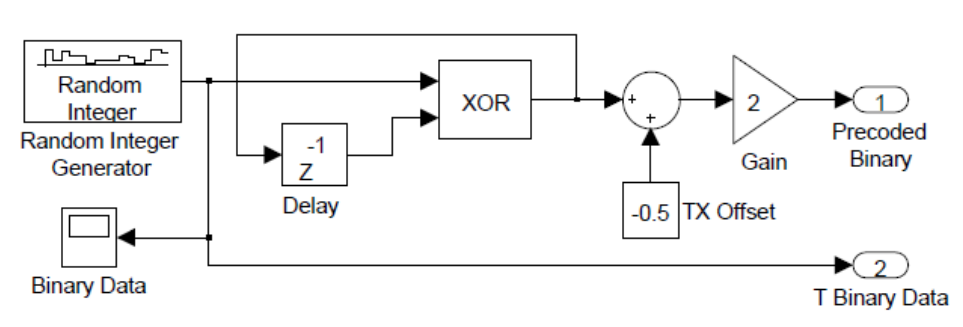
\includegraphics[scale=0.5]{simdbprecode}
  \label{fig:simmdbprecode}
\end{figure}

O sistema de pré-codificação modificado da figura \ref{fig:simmdbprecode} tem os parâmetros descritos abaixo.

\textbf{A – Integer Delay} – Signal Processing blockset; Signal Operations

PARÂMETROS: - Number of delays: 2; Input processing: Inherited; Initial conditions: 0.0; Sample time: -1.

Os parâmetros de simulação são:

\begin{lstlisting}[language=matlab]
Configuration Parameters: 
Start time: 0; 
Stop time: 0.05; 
Type: Fixed-step; 
Solver: ode3;  
Fixed-step size: 2e-5; 
Periodic sample time constraint: Unconstrained; 
Tasking mode for periodic sample times: Auto.
\end{lstlisting}

Obeter:
\begin{enumerate}
  \item gráfico nos pontos onde possui o osciloscópio. Explicar o seu funcionamento através da comparação entre gráficos;
  
  \item verificar o atraso no sinal recebido em relação ao transmitido;
  
   \item preencher a tabela \ref{tab:simmdb} com os dados da simulação;
  
  \item plotar o gráfico BERxSNR com um LPF (9 polos Chebyshev, 0,1 dB de ripple, freq. Corte de 600 Hz) em um sistema de comunicação digital PAM sinc duobinário precodificado com potência do sinal normalizada 50,6W;
  
  \item comparar o desempenho com o sistema duobinário.
\end{enumerate}

\begin{table}[H]
  \begin{center}
    \caption{Tabela BER x Eb/No para PAM duobinário modificado.}
    \begin{tabular}{|c|c|c|}
      \hline
      SNR (dB) & AWGN $\sigma^2 (V^2)$ & BER \\
      \hline
      7,01 & 10 & 0 \\
      \hline
      & 50 &  \\
      \hline
      & 100 & 0.0058 \\
      \hline
      & 200 & \\
      \hline
      & 300 & \\
      \hline
      & 400 & \\
      \hline 
      & 500 & \\
      \hline
    \end{tabular}
    \label{tab:simmdb}
  \end{center}
\end{table}

\subsubsection{Densidade Espectral de Potência (PSD) dos PAM Duobinários}

Obter a densidade espectral de potência (PSD) para os sistemas PAM duobinário e duobinário modificado (blocos das figuras \ref{fig:simdbpsd} e \ref{fig:simmdbpsd}, respectivamente).

\begin{figure}[H]
  \centering
  \caption{PSD PAM duobinário.}
  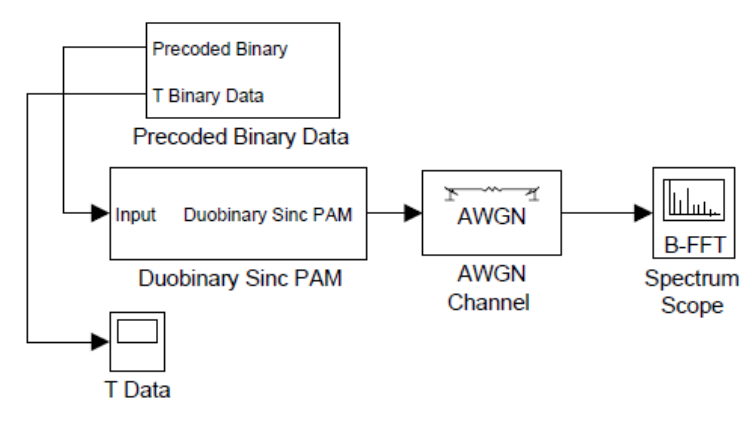
\includegraphics[scale=0.3]{simdbpsd}
  \label{fig:simdbpsd}
\end{figure}

\begin{figure}[H]
  \centering
  \caption{PSD PAM duobinário modificado.}
  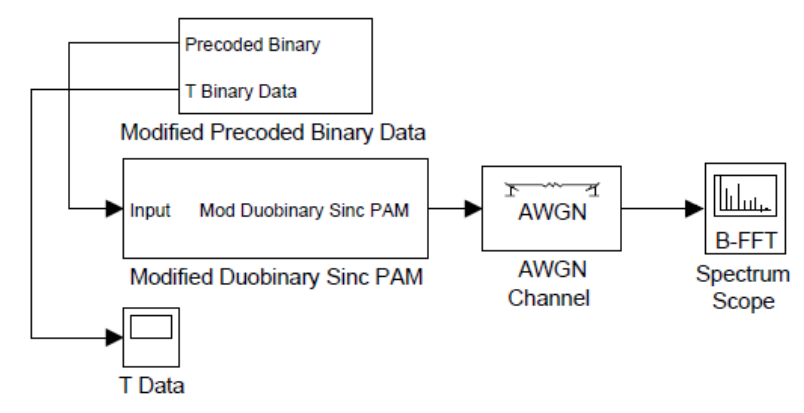
\includegraphics[scale=0.3]{simmdbpsd}
  \label{fig:simmdbpsd}
\end{figure}

Os parâmetros do bloco são:

\textbf{A – Spectrum Scope} – Signal Processing Blockset; Signal Processing Sinks

PARÂMETROS: Scope Properties: Spectrum units: dBW/Hertz; Spectrum type: One-sided; [x] Buffer input; Buffer size: 262144; Buffer overlap: 0; Treat Mx1and ....: M channels; Window: Boxcar; [x] Specify FFT length; Number of spectral averages: 1; FFT length: 262144. Axis Properties: [x] Inherit sample....; Frequency display offset (Hz): 0; Frequancy display limits: Auto; MinimumY-limit: -100; Maximum Y-limit: 10; Y-Axis label: Power Spectrum dB.

Os parâmetros de simulação são:

\begin{lstlisting}[language=matlab]
Configuration Parameters: 
Start time: 0; 
Stop time: 5.24288; 
Type: Fixed-step;
Solver: ode3; 
Fixed-step size: 2e-5; 
Periodic sample time constraint: Unconstrained; 
Tasking mode for periodic sample times: Auto.
\end{lstlisting}